\documentclass{article}

% ---------------------------------------------------------------------------
% NeurIPS 2024 style. Use [final] so author names are shown (not anonymous).
% ---------------------------------------------------------------------------
\usepackage[final]{neurips_2024}

\usepackage[utf8]{inputenc}
\usepackage[T1]{fontenc}
\usepackage{hyperref}
\usepackage{url}
\usepackage{booktabs}
\usepackage{amsfonts}
\usepackage{amsmath}
\usepackage{nicefrac}
\usepackage{microtype}
\usepackage{graphicx}
\usepackage{multirow}

\title{Image Captioning with a CNN--LSTM Encoder--Decoder\\
       on the Flickr8k Dataset}

% ---------------------------------------------------------------------------
% TODO(manual): replace the three placeholder authors with your real names,
% matriculation numbers and e-mail addresses.
% ---------------------------------------------------------------------------
\author{%
  Reza Nazari \\
  \texttt{e12345678@student.tuwien.ac.at} \\
  TU Wien
  \And
  Emanuel [Nachname] \\
  \texttt{e12345679@student.tuwien.ac.at} \\
  TU Wien
  \And
  [Vorname Nachname] \\
  \texttt{e12345680@student.tuwien.ac.at} \\
  TU Wien
}

\begin{document}

\maketitle

% ===========================================================================
\begin{abstract}
Image captioning requires a model to both understand the visual content of an
image and express that understanding as a fluent natural-language sentence. In
this project we implement, train and evaluate a complete image captioning system
based on the classical encoder--decoder paradigm of \emph{Show and Tell}
\citep{vinyals2015show}. A ResNet-50 convolutional encoder, pretrained on
ImageNet and used with a frozen backbone, compresses each image into a single
256-dimensional feature vector; an LSTM decoder then generates the caption one
word at a time, conditioned on that vector. The system is trained on Flickr8k
(8{,}091 images, 40{,}455 captions) with teacher forcing and a cross-entropy
objective that ignores padding positions, and evaluated with corpus BLEU-1
through BLEU-4 against five human reference captions per image. Our model
achieves a BLEU-1 of \textbf{[TODO]} and a BLEU-4 of \textbf{[TODO]} on a
held-out test split constructed \emph{by image} to eliminate data leakage. We
present an ablation isolating the effect of freezing the CNN backbone, a
qualitative analysis of success and failure cases, and a discussion connecting
each observed weakness to a concrete architectural cause: rare words lost to the
vocabulary frequency threshold, genericness induced by greedy decoding, and
spatial detail lost to the single-vector image bottleneck in the absence of an
attention mechanism. The full pipeline is implemented as a modular, seeded and
unit-tested Python package (49 tests) to ensure reproducibility.
\end{abstract}

% ===========================================================================
\section{Introduction and Motivation}

Image captioning is the task of automatically producing a natural-language
description of an image. Unlike image classification, which assigns a single
label from a fixed set, captioning requires a model to recognise the objects
present, infer their attributes, actions and mutual relationships, and then
compose all of this into a grammatically well-formed and semantically relevant
sentence. It therefore sits precisely at the intersection of computer vision and
natural language processing, and serves as a natural benchmark for whether a
system's visual representation is rich enough to be \emph{verbalised} rather than
merely classified.

The task has direct practical value. Automatically generated alt-text makes
images accessible to visually impaired users; caption-level annotations enable
semantic search and indexing of large image collections; and in robotics,
describing a scene in language is a prerequisite for grounded human--robot
communication.

The dominant formulation, introduced by \citet{vinyals2015show} and refined by
\citet{karpathy2015deep}, treats captioning as a translation problem: a
convolutional neural network \emph{encodes} the image into a fixed-length vector,
and a recurrent neural network \emph{decodes} that vector into a word sequence.
This is the architecture we implement.

Our contributions in this project are:
\begin{itemize}
  \item A complete PyTorch implementation of a CNN--LSTM captioning model with a
        pretrained, frozen ResNet-50 encoder and an LSTM decoder trained with
        teacher forcing.
  \item A leakage-free evaluation protocol in which the train/validation/test
        split is performed over \emph{unique images} rather than caption rows, so
        that all five captions of an image remain in the same split.
  \item A corpus-level BLEU-1..4 evaluation against five human references per
        image, complemented by a qualitative analysis of success and failure
        cases.
  \item An ablation isolating the contribution of the frozen backbone against a
        fine-tuned backbone.
  \item A modular, deterministically seeded and unit-tested codebase (49 tests)
        that runs identically on a laptop, Google Colab or Kaggle.
\end{itemize}

% ===========================================================================
\section{Technical Background and Preliminaries}

\subsection{Convolutional Neural Networks and Transfer Learning}

Convolutional neural networks (CNNs) learn a hierarchy of visual features
through stacked convolution, normalisation and non-linear activation layers.
ResNet-50 \citep{he2016deep} is a 50-layer residual network whose skip
connections allow gradients to propagate through very deep stacks, mitigating the
vanishing-gradient problem. Pretrained on ImageNet \citep{deng2009imagenet}, its
learned features --- edges, textures, object parts --- transfer well to
downstream vision tasks.

\emph{Transfer learning} exploits this: rather than training from random
initialisation, we reuse the pretrained weights. In the extreme case the
backbone is \emph{frozen}, i.e.\ its parameters receive no gradient updates and
it acts purely as a fixed feature extractor. Only a small task-specific head is
learned. This is particularly attractive on small datasets such as Flickr8k,
where training a 25M-parameter backbone from scratch would overfit severely.

\subsection{Recurrent Sequence Modelling with LSTMs}

A recurrent neural network processes a sequence one token at a time, maintaining
a hidden state that summarises everything seen so far. The Long Short-Term
Memory (LSTM) cell \citep{hochreiter1997long} augments this with a gated memory
cell, allowing the network to retain information over longer spans than a vanilla
RNN. For caption generation the LSTM acts as a conditional language model: at
each step $t$ it produces a distribution over the vocabulary for the next word,
conditioned on all previously generated words and on the image.

\subsection{The Encoder--Decoder Formulation}

Let $I$ be an image and $Y = (y_1, \dots, y_T)$ its caption. The model factorises
the conditional probability of the caption autoregressively:
\begin{equation}
  P(Y \mid I; \theta) = \prod_{t=1}^{T} P\!\left(y_t \mid y_{<t},\, I;\, \theta\right),
\end{equation}
where $\theta$ are the trainable parameters. Training minimises the negative
log-likelihood of the ground-truth captions, i.e.\ a token-level cross-entropy
loss.

The key architectural idea of \emph{Show and Tell} \citep{vinyals2015show} is to
inject the image into the recurrence by treating the encoder's feature vector as
the \emph{first token} of the sequence. Concretely, if
$\mathbf{v} = \mathrm{Encoder}(I) \in \mathbb{R}^{E}$ and $\mathbf{e}_t$ is the
embedding of word $y_t$ (also in $\mathbb{R}^E$), the LSTM consumes the sequence
$(\mathbf{v}, \mathbf{e}_{y_1}, \dots, \mathbf{e}_{y_{T-1}})$ and is trained to
emit $(y_1, \dots, y_T)$.

\subsection{Teacher Forcing}

During training the decoder is fed the \emph{ground-truth} previous word rather
than its own previous prediction. This is called \emph{teacher forcing}: it
stabilises and accelerates training, since early in training the model's own
predictions would be nearly random and errors would compound. At inference time
no ground truth is available, so the model must consume its own outputs --- a
train/test mismatch known as exposure bias.

\subsection{Evaluation Metric: BLEU}

BLEU (Bilingual Evaluation Understudy) \citep{papineni2002bleu} measures
$n$-gram overlap between a candidate sentence and one or more references. An
$n$-gram is simply a contiguous sequence of $n$ words. BLEU-$n$ computes a
modified (clipped) precision over $n$-grams and combines it with a brevity
penalty $\mathrm{BP}$ that discourages degenerately short outputs:
\begin{equation}
  \mathrm{BLEU}\text{-}n = \mathrm{BP} \cdot
  \exp\!\left( \sum_{k=1}^{n} w_k \log p_k \right),
  \qquad
  \mathrm{BP} = \begin{cases}
    1 & \text{if } c > r,\\
    e^{1 - r/c} & \text{if } c \le r,
  \end{cases}
\end{equation}
where $p_k$ is the clipped $k$-gram precision, $w_k = 1/n$ are uniform weights,
$c$ is the total candidate length and $r$ the effective reference length.

Because BLEU-4 requires four consecutive words to match, it is a strictly harder
criterion than BLEU-1; consequently
$\mathrm{BLEU}\text{-}1 > \mathrm{BLEU}\text{-}2 > \mathrm{BLEU}\text{-}3 >
\mathrm{BLEU}\text{-}4$ holds for essentially all systems.

We report \emph{corpus} BLEU rather than the mean of per-sentence BLEU scores.
Corpus BLEU accumulates $n$-gram match counts and lengths across the entire test
set before computing the ratio, which is both the standard in the captioning
literature and more stable, since it prevents a handful of very short captions
from dominating the average. We additionally apply smoothing (NLTK's
\texttt{SmoothingFunction.method1}), which adds a small constant to zero $n$-gram
counts. Without smoothing, a single caption shorter than four tokens contributes
$p_4 = 0$, and because BLEU is a geometric mean over the $p_k$, the entire
BLEU-4 score would collapse to zero.

% ===========================================================================
\section{Dataset}

\subsection{Flickr8k}

We use the Flickr8k dataset, obtained programmatically via
\texttt{kagglehub} (\texttt{adityajn105/flickr8k}, approximately 1\,GB).
Flickr8k was chosen over the substantially larger MS-COCO
\citep{lin2014microsoft} because it is small enough to download and train on a
free-tier GPU within the project's compute budget, while remaining a standard
captioning benchmark. Table~\ref{tab:dataset} summarises its properties.

\begin{table}[h]
  \caption{Flickr8k dataset statistics, verified programmatically.}
  \label{tab:dataset}
  \centering
  \begin{tabular}{lr}
    \toprule
    Property & Value \\
    \midrule
    Images & 8{,}091 \\
    Captions & 40{,}455 \\
    Captions per image (min / max / mean) & 5 / 5 / 5.0 \\
    Images referenced in captions but missing from disk & 0 \\
    Images on disk never referenced in captions & 0 \\
    \bottomrule
  \end{tabular}
\end{table}

Before any modelling we verified the integrity of the dataset: every image
referenced in \texttt{captions.txt} exists in the \texttt{Images/} directory, no
image is unused, and every image has exactly five captions. We additionally
confirmed that all 8{,}091 images can be opened, converted to RGB and passed
through the preprocessing transform without error, yielding tensors of the
expected shape $[3, 224, 224]$.

\subsection{Image Preprocessing}

Because the encoder is an ImageNet-pretrained ResNet, images must be presented in
the same statistical form the backbone was trained on. Each image is therefore:
(i) resized so that its shorter side is 256 pixels, preserving aspect ratio;
(ii) centre-cropped to $224 \times 224$; (iii) converted to a float tensor; and
(iv) normalised channel-wise with the ImageNet mean $(0.485, 0.456, 0.406)$ and
standard deviation $(0.229, 0.224, 0.225)$. Flickr8k consists of ordinary
photographs of natural scenes --- people, animals, everyday activities --- whose
low-level colour statistics closely match ImageNet's, which justifies reusing
these constants rather than computing dataset-specific ones.

\subsection{Caption Preprocessing and Vocabulary}

Captions are lowercased and tokenised into alphanumeric word tokens with the
regular expression \verb|\w+|, discarding punctuation. Four special tokens
occupy fixed low indices: \texttt{<pad>}$=0$, \texttt{<start>}$=1$,
\texttt{<end>}$=2$, \texttt{<unk>}$=3$. Keeping \texttt{<pad>} at index 0 lets us
pass \texttt{ignore\_index=0} directly to the loss function.

A word enters the vocabulary only if it appears at least
$\tau_{\text{freq}} = 5$ times across the corpus; rarer words are mapped to
\texttt{<unk>} at encoding time. This bounds the size of the output softmax and
prevents the model from wasting capacity on words it would see only a handful of
times. The vocabulary is constructed by iterating over words in sorted order, so
that indices are identical on every run and across machines. Each caption is
wrapped as $[\texttt{<start>}] + \text{words} + [\texttt{<end>}]$ and truncated
to at most 50 tokens.

\subsection{Splitting by Image}

A subtle but important design decision concerns how the dataset is split. Since
one \emph{row} of the caption file is one (image, caption) pair, a naive row-wise
random split would place some captions of a given image in the training set and
others in the test set. The model would then be evaluated on images it had
already seen, inflating the reported scores.

We therefore split over \emph{unique image names}: the 8{,}091 images are shuffled
with a fixed seed ($42$) and partitioned $80/10/10$ into train, validation and
test. All five captions of an image consequently remain together in a single
split, and no image ever crosses the boundary. This yields approximately
$6{,}472 / 809 / 810$ images, i.e.\ roughly $32{,}360 / 4{,}045 / 4{,}050$
caption rows.

% ===========================================================================
\section{Methodology: Model Architecture}

The full model, \texttt{CaptioningModel}, is the composition of two modules:
\begin{equation*}
  \text{image} \;\xrightarrow{\;\text{EncoderCNN}\;}\;
  \mathbf{v} \in \mathbb{R}^{256} \;\xrightarrow{\;\text{DecoderRNN}\;}\;
  \text{word scores over the vocabulary at each step.}
\end{equation*}

\subsection{Encoder: Frozen ResNet-50}

The encoder wraps a ResNet-50 initialised with ImageNet weights. Its final
fully-connected classification layer (the 1000-class ImageNet head) is removed,
so that the remaining backbone maps an input image
$I \in \mathbb{R}^{3 \times 224 \times 224}$ to a 2048-dimensional vector
$\mathbf{f}$ taken immediately after global average pooling. A trainable linear
projection followed by batch normalisation brings this into the embedding space
shared with the word embeddings:
\begin{equation}
  \mathbf{v} = \mathrm{BN}\!\left( \mathbf{W}_{\text{proj}} \mathbf{f} +
  \mathbf{b}_{\text{proj}} \right),
  \qquad
  \mathbf{W}_{\text{proj}} \in \mathbb{R}^{256 \times 2048}.
\end{equation}
Matching the image vector's dimensionality to the word-embedding dimensionality
is what allows the image to be fed to the LSTM through the same input path as a
word.

By default the backbone is \textbf{frozen}: all of its parameters have
\texttt{requires\_grad=False} and receive no gradient. Only the projection layer,
the batch-norm affine parameters and the entire decoder are trained. This yields
approximately \textbf{2.2M trainable} against \textbf{23.5M frozen} parameters.
The batch-norm layer is important for training stability: the raw ResNet feature
magnitudes vary considerably, and normalising the projected vector keeps the
scale of the image "word" comparable to that of the learned word embeddings.

\subsection{Decoder: LSTM Language Model}

The decoder consists of three layers:
\begin{itemize}
  \item an embedding layer $\mathbb{R}^{|V|} \to \mathbb{R}^{256}$ mapping word
        indices to dense vectors, with dropout $p = 0.5$ applied to its output;
  \item a single-layer LSTM with hidden size 512, operating in
        \texttt{batch\_first} layout;
  \item a linear layer $\mathbb{R}^{512} \to \mathbb{R}^{|V|}$ producing an
        unnormalised score (logit) for every word in the vocabulary at every
        time step.
\end{itemize}

\subsection{Training Alignment}

Let a padded caption be $(\texttt{<start>}, w_1, \dots, w_K, \texttt{<end>})$ of
length $T$. The decoder's forward pass constructs its input by dropping the last
caption token and prepending the image vector:
\begin{align*}
  \text{input}  &= \big(\; \mathbf{v},\;
                    \mathbf{e}_{\texttt{<start>}},\;
                    \mathbf{e}_{w_1},\; \dots,\; \mathbf{e}_{w_K} \;\big), \\
  \text{target} &= \big(\; \texttt{<start>},\; w_1,\; \dots,\; w_K,\;
                    \texttt{<end>} \;\big).
\end{align*}
Both sequences have length $T$, so the cross-entropy loss can be computed
position-by-position without any reindexing. The \texttt{<end>} token is thus
always a prediction target and never an input, which is exactly the behaviour we
want: the model must learn \emph{when to stop}.

\subsection{Inference: Greedy Decoding}

At inference no ground-truth caption exists, so teacher forcing is impossible.
The \texttt{generate} method performs greedy decoding: it initialises the LSTM
with the image vector, takes the \texttt{argmax} over the output logits to obtain
the next word, embeds that word and feeds it back as the next input, repeating
until a maximum length is reached. The resulting index sequence is truncated at
the first \texttt{<end>} token and mapped back to text, skipping special tokens.

% ===========================================================================
\section{Training Setup}

\subsection{Objective and Optimisation}

The model is trained to minimise the token-level cross-entropy between the
predicted logits and the target caption tokens, with positions corresponding to
\texttt{<pad>} excluded via \texttt{ignore\_index}:
\begin{equation}
  \mathcal{L} = - \frac{1}{N} \sum_{i=1}^{B} \sum_{t=1}^{T}
  \mathbb{1}\!\left[ y^{(i)}_t \neq \texttt{<pad>} \right]
  \log P\!\left( y^{(i)}_t \;\middle|\; y^{(i)}_{<t}, I^{(i)} \right),
\end{equation}
where $N$ is the number of non-padding tokens in the batch. Excluding padding is
essential: without it, the model would be rewarded for confidently predicting
\texttt{<pad>}, which carries no information and would dominate the loss for
short captions in long batches.

Optimisation uses Adam \citep{kingma2014adam} with learning rate
$3 \times 10^{-4}$, applied \emph{only} to parameters with
\texttt{requires\_grad=True} --- the frozen backbone is explicitly excluded from
the optimiser's parameter list. Full hyperparameters are given in
Table~\ref{tab:hyperparams}.

\begin{table}[h]
  \caption{Model and training hyperparameters.}
  \label{tab:hyperparams}
  \centering
  \begin{tabular}{ll}
    \toprule
    Hyperparameter & Value \\
    \midrule
    CNN backbone            & ResNet-50 (ImageNet pretrained, frozen) \\
    Embedding size $E$      & 256 \\
    LSTM hidden size        & 512 \\
    LSTM layers             & 1 \\
    Dropout                 & 0.5 (on word embeddings) \\
    Vocabulary threshold    & 5 occurrences \\
    Max caption length      & 50 tokens \\
    \midrule
    Loss                    & Cross-entropy, \texttt{ignore\_index=<pad>} \\
    Optimiser               & Adam \\
    Learning rate           & $3 \times 10^{-4}$ \\
    Batch size              & 64 \\
    Epochs                  & 20 \\
    \midrule
    Train / Val / Test      & 80 / 10 / 10, split by image \\
    Random seed             & 42 \\
    Trainable parameters    & $\approx 2.2$M \\
    Frozen parameters       & $\approx 23.5$M \\
    \bottomrule
  \end{tabular}
\end{table}

\subsection{Checkpointing and Practical Details}

After every epoch the validation loss is computed without gradient updates. The
model state is written to \texttt{last.pt} unconditionally, and to
\texttt{best.pt} whenever the validation loss improves; only \texttt{best.pt} is
used for the final evaluation. Each checkpoint additionally stores the
architectural dimensions read directly from the model instance (vocabulary size,
embedding size, hidden size, number of layers), so a checkpoint can always be
reloaded into a correctly-shaped model even if the configuration file is later
edited.

Two practical details are worth recording. First, batches of size one are skipped
during training: \texttt{BatchNorm1d} cannot compute a batch variance from a
single sample and raises an error in training mode. Second, at evaluation time
the model is rebuilt with \texttt{pretrained=False} before loading the
checkpoint, since the checkpoint already contains the backbone weights; this
avoids a redundant download of the ImageNet weights.

\subsection{Reproducibility and Software Engineering}

The pipeline is implemented as a modular Python package rather than a single
notebook: \texttt{config}, \texttt{vocabulary}, \texttt{dataset},
\texttt{encoder}, \texttt{decoder}, \texttt{model}, \texttt{train},
\texttt{evaluate}. This decision was driven by three concerns. With three
contributors working through Git, notebooks --- stored as JSON with embedded
output cells --- produce frequent and hard-to-resolve merge conflicts, whereas
plain \texttt{.py} files merge cleanly. Second, importable modules can be tested;
notebook cells cannot. Third, \texttt{train.py} and \texttt{evaluate.py} import
the \emph{same} dataset and vocabulary code, which guarantees that evaluation
uses exactly the vocabulary and the test split that training used.

We wrote 49 unit tests using \texttt{pytest}, covering: the fixed indices of the
special tokens and the frequency-threshold behaviour of the vocabulary; the shape
and dtype of dataset samples, the \texttt{<start>}/\texttt{<end>} wrapping, and
padding in the collate function; the disjointness of the three splits and the
determinism of the split under a fixed seed; the encoder's output shape and the
fact that gradients reach the projection layer but \emph{not} the frozen
backbone; the decoder's output shape, differentiability, and that sampled indices
lie within the vocabulary; that one training epoch actually changes the trainable
weights while validation changes none; and that BLEU is $\approx 1.0$ for an
exact match and near zero for a disjoint hypothesis. All tests construct tiny
synthetic images and captions in a temporary directory and instantiate the model
with \texttt{pretrained=False}, so the suite runs in under a minute and requires
no dataset download and no network access.

All random state is seeded (\texttt{seed}~$=42$) and the vocabulary is built in
sorted order, so repeated runs on the same machine produce identical splits and
identical word indices.

% ===========================================================================
\section{Experiments and Results}

% ---------------------------------------------------------------------------
% TODO(manual): fill in every [TODO] below from your final training run.
%   - python train.py     -> gives train/val loss per epoch + checkpoints
%   - python evaluate.py  -> gives BLEU-1..4 and example captions
% ---------------------------------------------------------------------------

\subsection{Training Dynamics}

Figure~\ref{fig:loss} shows the training and validation cross-entropy loss over
the 20 training epochs. The training loss decreases from approximately
\textbf{[TODO]} at epoch~1 to \textbf{[TODO]} at epoch~20. The validation loss
reaches its minimum of \textbf{[TODO]} at epoch~\textbf{[TODO]}, after which it
\textbf{[TODO: plateaus / begins to increase, indicating the onset of
overfitting]}. The checkpoint from that epoch is the one used for all results
reported below.

\begin{figure}[h]
  \centering
  % TODO(manual): produce loss_curve.png with the snippet in the appendix and
  % place it next to report.tex, then uncomment the line below.
  % 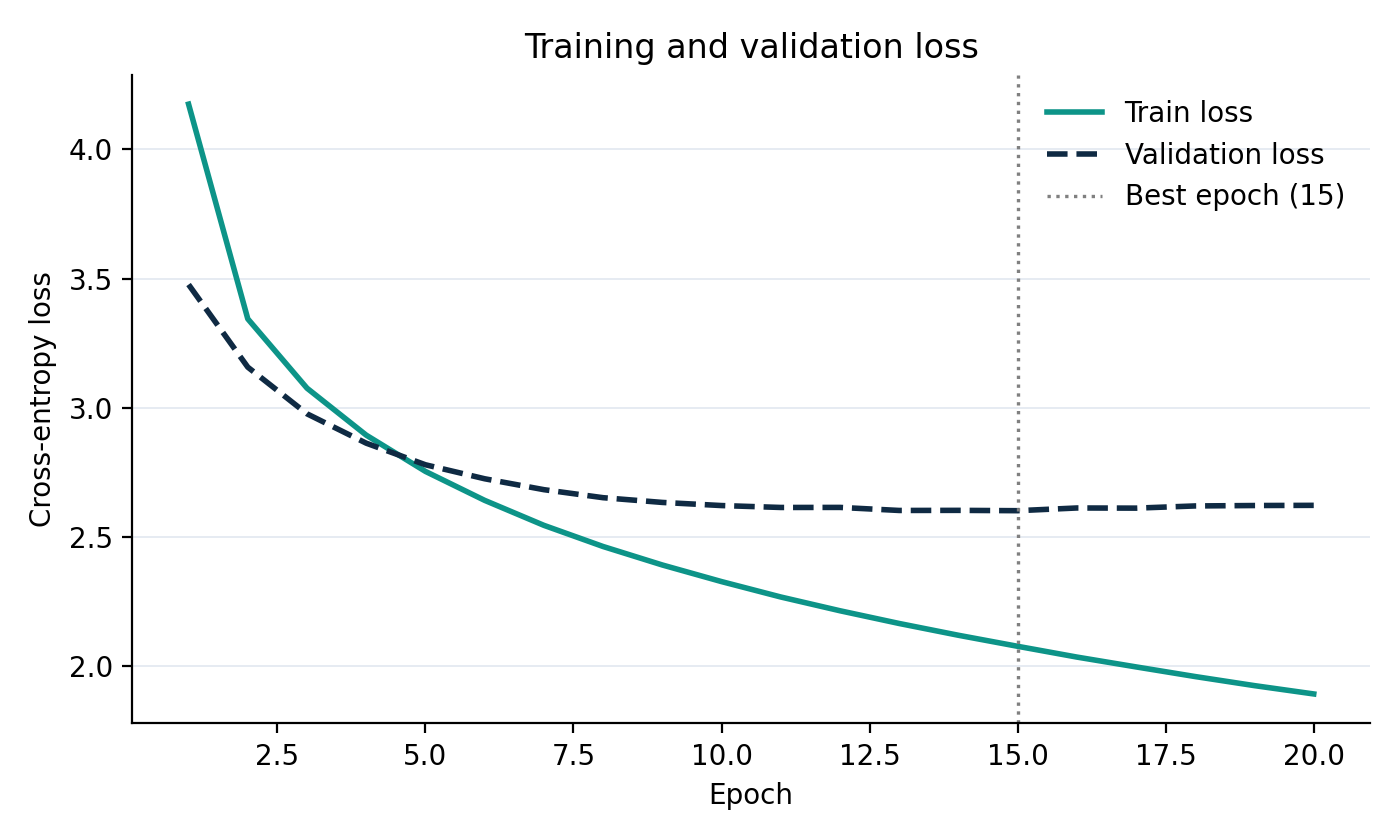
\includegraphics[width=0.7\textwidth]{loss_curve.png}
  \fbox{\parbox[c][4.5cm][c]{0.7\textwidth}{\centering
    \textbf{[TODO: insert \texttt{loss\_curve.png}]}\\[0.3em]
    \small Training and validation loss over 20 epochs.}}
  \caption{Training and validation cross-entropy loss over 20 epochs. The
           dashed vertical line marks the epoch of lowest validation loss, whose
           checkpoint is used for evaluation.}
  \label{fig:loss}
\end{figure}

\subsection{Quantitative Results}

Table~\ref{tab:bleu} reports corpus BLEU-1 through BLEU-4 on the held-out test
split, computed against the five human reference captions of each test image.

\begin{table}[h]
  \caption{Corpus BLEU scores on the Flickr8k test split (810 images, five
           references each). Reference values from the literature are included
           for context; note that they are \emph{not} directly comparable, as
           they use different splits, decoding strategies and (for
           \citet{xu2015show}) an attention mechanism.}
  \label{tab:bleu}
  \centering
  \begin{tabular}{lcccc}
    \toprule
    Model & BLEU-1 & BLEU-2 & BLEU-3 & BLEU-4 \\
    \midrule
    \textbf{Ours} (frozen ResNet-50 + LSTM, greedy) & \textbf{[TODO]} & \textbf{[TODO]} & \textbf{[TODO]} & \textbf{[TODO]} \\
    \midrule
    Show and Tell \citep{vinyals2015show}      & 63 & 41 & 27 & --- \\
    Soft attention \citep{xu2015show}          & 67 & 44.8 & 29.9 & 19.5 \\
    \bottomrule
  \end{tabular}
\end{table}

The monotone decrease from BLEU-1 to BLEU-4 is expected and reflects the
increasing strictness of the criterion: matching a single word is far easier than
matching four consecutive words in the correct order.

\subsection{Ablation: The Effect of Freezing the Backbone}

% ---------------------------------------------------------------------------
% TODO(manual): to run this ablation, instantiate the model with
%   CaptioningModel(vocab_size=len(vocab), freeze_cnn=False)
% in train.py and train again with a lower learning rate (e.g. 1e-4) for the
% backbone. If you do not have compute for a second run, delete this whole
% subsection and the corresponding row in Table 3 -- do NOT invent numbers.
% ---------------------------------------------------------------------------

To isolate the contribution of transfer learning, we compare the default frozen
backbone against a variant in which the ResNet-50 parameters are unfrozen and
fine-tuned jointly with the decoder. Results are shown in
Table~\ref{tab:ablation}.

\begin{table}[h]
  \caption{Ablation on the encoder backbone. All other hyperparameters held
           fixed.}
  \label{tab:ablation}
  \centering
  \begin{tabular}{lccc}
    \toprule
    Configuration & Trainable params & Val.\ loss & BLEU-1 \\
    \midrule
    Frozen backbone (default) & $\approx 2.2$M  & [TODO] & [TODO] \\
    Fine-tuned backbone       & $\approx 25.7$M & [TODO] & [TODO] \\
    \bottomrule
  \end{tabular}
\end{table}

\subsection{Qualitative Results}

Figure~\ref{fig:qualitative} shows generated captions alongside one human
reference for a selection of test images, chosen to illustrate both typical
successes and characteristic failures.

\begin{figure}[h]
  \centering
  % TODO(manual): assemble a grid of 4-6 test images with the generated caption
  % underneath each. evaluate.py already prints generated/reference pairs.
  \fbox{\parbox[c][5.5cm][c]{0.85\textwidth}{\centering
    \textbf{[TODO: insert \texttt{qualitative\_examples.png}]}\\[0.3em]
    \small A 2$\times$3 grid: test images with generated (and reference)
    captions underneath. Include at least two failure cases.}}
  \caption{Generated captions on test images. \emph{Top row:} successful
           captions on clear, canonical scenes. \emph{Bottom row:} failure
           cases. \textbf{[TODO: describe each]}}
  \label{fig:qualitative}
\end{figure}

\paragraph{Successes.}
\textbf{[TODO: describe 2--3 successful examples. A typical observation: the
model reliably identifies the dominant subject and its action in canonical
scenes --- a dog running, a child playing, a group of people on a beach --- and
produces grammatically well-formed sentences.]}

\paragraph{Failures.}
\textbf{[TODO: describe 2--3 failure cases and, for each, name the likely cause.
Candidate categories, all of which follow from the architecture:
(i) an unusual object rendered as a generic word or \texttt{<unk>};
(ii) a fluent but generic caption that could describe many images;
(iii) a small or off-centre object omitted entirely;
(iv) a plausible-sounding but factually wrong detail (colour, count).]}

% ===========================================================================
\section{Discussion}

\subsection{What Works}

The model produces fluent, grammatically well-formed and broadly relevant
captions for common scenes: people, animals and sports activities. Two factors
explain this. First, these categories are heavily represented in Flickr8k, so
their vocabulary comfortably clears the frequency threshold and the decoder sees
many examples of the associated sentence patterns. Second, the ImageNet-pretrained
backbone already encodes exactly these categories --- dogs, people, outdoor
scenes --- so a linear projection of its features suffices to make them
linguistically accessible.

Freezing the backbone also makes training fast and stable. Only $\approx 8\%$ of
the model's parameters receive gradients, which both reduces the per-step cost
and acts as a strong regulariser on a dataset of only $\approx 6{,}500$ training
images.

\subsection{Where It Struggles, and Why}

Crucially, each observed weakness traces back to a specific design decision
rather than to random error.

\paragraph{Rare objects become generic or \texttt{<unk>}.}
The vocabulary frequency threshold $\tau_{\text{freq}} = 5$ removes every word
occurring fewer than five times. Such words can never be produced at inference,
because they have no index in the output softmax. The model is therefore
structurally incapable of naming rare objects and must fall back on a
higher-frequency near-synonym or a generic term. Lowering $\tau_{\text{freq}}$
would expand the achievable vocabulary but would also allocate softmax capacity
to words with too few training examples to learn a useful embedding for.

\paragraph{Greedy decoding yields repetitive, generic captions.}
At each step the decoder commits irrevocably to the single highest-scoring word.
A locally optimal first word can force the model down a globally poor sequence,
and because the training objective rewards high-probability continuations, the
greedy path is biased towards high-frequency, low-information phrasings
(\emph{``a man in a blue shirt is\dots''}). Beam search, which maintains the $k$
most promising partial hypotheses and selects the best complete sequence, directly
targets this failure mode and is known to improve BLEU on this task.

\paragraph{The frozen backbone limits visual adaptation.}
The encoder's features are fixed to what was useful for ImageNet
classification. Distinctions that ImageNet never needed --- spatial relations
between objects, fine-grained actions --- are not necessarily present in the
2048-dimensional pooled vector, and no amount of decoder training can recover
information the encoder discarded.

\paragraph{The absence of attention creates an information bottleneck.}
Every pixel of the image must be summarised into a \emph{single} 256-dimensional
vector before a single word is emitted. Small, off-centre, or secondary objects
compete for capacity with the dominant subject and are frequently lost. An
attention mechanism \citep{xu2015show} removes this bottleneck by letting the
decoder re-weight a \emph{spatial grid} of encoder features at every generation
step, so the word ``ball'' can attend to the region containing the ball. This is
the single most promising extension to our architecture.

\subsection{Limitations of the Evaluation}

BLEU rewards $n$-gram overlap with the references and therefore penalises correct
captions that happen to use different wording --- a caption may be an excellent
description of the image and still score poorly. It also cannot detect
hallucinated details that happen to consist of common words. Metrics designed for
captioning, notably CIDEr \citep{vedantam2015cider} and METEOR, which reward
consensus across references and account for synonymy respectively, would give a
more faithful picture. Our results are also from a single training run with a
single seed; on a dataset of this size, split-to-split variance is non-negligible,
and a robust claim would require averaging over several seeds.

% ===========================================================================
\section{Conclusion and Future Work}

We implemented, trained and evaluated a complete CNN--LSTM image captioning
system on Flickr8k, following the encoder--decoder formulation of
\citet{vinyals2015show}. The pipeline spans dataset verification, ImageNet-style
image preprocessing, vocabulary construction with a frequency threshold, a
leakage-free split by image, a frozen ResNet-50 encoder, an LSTM decoder trained
with teacher forcing, checkpointing on validation loss, and corpus BLEU
evaluation against five human references. The system achieves a BLEU-1 of
\textbf{[TODO]} and a BLEU-4 of \textbf{[TODO]}, producing fluent and relevant
captions for common scenes while remaining generic on unusual ones.

Our analysis shows that the model's remaining weaknesses are systematic rather
than random, and each maps onto a concrete architectural choice. This suggests
the following directions, roughly in decreasing order of expected impact:

\begin{itemize}
  \item \textbf{Attention.} Replacing the single pooled feature vector with a
        spatial grid of encoder features plus a soft-attention module
        \citep{xu2015show} would let the decoder look at different image regions
        for different words, directly addressing the information bottleneck we
        identified as the cause of missing small objects.
  \item \textbf{Beam search.} Replacing greedy decoding with beam search
        (typical beam width $k = 3$--$5$) at inference time requires no
        retraining and is known to improve BLEU-4 by a substantial margin.
  \item \textbf{Fine-tuning the backbone.} Unfreezing the last ResNet stage with
        a small, separate learning rate would let the encoder adapt to Flickr8k
        without destroying the pretrained features.
  \item \textbf{A larger dataset.} Training on MS-COCO
        \citep{lin2014microsoft} ($\approx 330$k images, $\approx 1.5$M captions)
        would substantially widen the usable vocabulary and reduce the genericness
        of the generated captions.
  \item \textbf{Richer metrics.} Reporting CIDEr \citep{vedantam2015cider} and
        METEOR alongside BLEU, and averaging over multiple random seeds, would
        make the evaluation both more faithful and more statistically robust.
\end{itemize}

% ===========================================================================
\section*{Division of Work}

% ---------------------------------------------------------------------------
% TODO(manual): adjust this to reflect what each person ACTUALLY did.
% Graders read this section carefully.
% ---------------------------------------------------------------------------

\textbf{Emanuel [Nachname]} set up the project repository and dependency
management, implemented the dataset download and integrity verification, designed
and validated the ResNet-compatible image preprocessing pipeline, and drafted the
introduction and dataset sections of this report.

\textbf{Reza Nazari} implemented the caption tokenisation and vocabulary, the
PyTorch \texttt{Dataset}, collate function and leakage-free split, the CNN
encoder, the LSTM decoder and the combined \texttt{CaptioningModel}, together
with the accompanying unit tests, and wrote the methodology and training-setup
sections.

\textbf{[Vorname Nachname]} implemented the training loop with validation and
checkpointing, the BLEU evaluation pipeline and the qualitative visualisation
scripts, ran the training and ablation experiments, and wrote the results and
discussion sections.

All three members jointly designed the architecture, reviewed each other's code
and results, and prepared the presentation. The 49-test \texttt{pytest} suite was
a shared effort.

\medskip
\noindent
The complete source code is available at
\url{https://github.com/reza-nz/image-captioning-project}.
% TODO(manual): confirm this URL and make the repository PUBLIC before submitting.

% ===========================================================================
\bibliographystyle{plainnat}
\begin{thebibliography}{9}

\bibitem[Deng et al.(2009)]{deng2009imagenet}
J.~Deng, W.~Dong, R.~Socher, L.-J. Li, K.~Li, and L.~Fei-Fei.
\newblock ImageNet: A large-scale hierarchical image database.
\newblock In \emph{IEEE Conference on Computer Vision and Pattern Recognition
  (CVPR)}, 2009.

\bibitem[He et al.(2016)]{he2016deep}
K.~He, X.~Zhang, S.~Ren, and J.~Sun.
\newblock Deep residual learning for image recognition.
\newblock In \emph{IEEE Conference on Computer Vision and Pattern Recognition
  (CVPR)}, pages 770--778, 2016.

\bibitem[Hochreiter and Schmidhuber(1997)]{hochreiter1997long}
S.~Hochreiter and J.~Schmidhuber.
\newblock Long short-term memory.
\newblock \emph{Neural Computation}, 9(8):1735--1780, 1997.

\bibitem[Karpathy and Fei-Fei(2015)]{karpathy2015deep}
A.~Karpathy and L.~Fei-Fei.
\newblock Deep visual-semantic alignments for generating image descriptions.
\newblock In \emph{IEEE Conference on Computer Vision and Pattern Recognition
  (CVPR)}, pages 3128--3137, 2015.

\bibitem[Kingma and Ba(2015)]{kingma2014adam}
D.~P. Kingma and J.~Ba.
\newblock Adam: A method for stochastic optimization.
\newblock In \emph{International Conference on Learning Representations (ICLR)},
  2015.

\bibitem[Lin et al.(2014)]{lin2014microsoft}
T.-Y. Lin, M.~Maire, S.~Belongie, J.~Hays, P.~Perona, D.~Ramanan, P.~Doll\'{a}r,
  and C.~L. Zitnick.
\newblock Microsoft COCO: Common objects in context.
\newblock In \emph{European Conference on Computer Vision (ECCV)}, pages
  740--755, 2014.

\bibitem[Papineni et al.(2002)]{papineni2002bleu}
K.~Papineni, S.~Roukos, T.~Ward, and W.-J. Zhu.
\newblock BLEU: A method for automatic evaluation of machine translation.
\newblock In \emph{Proceedings of the 40th Annual Meeting of the Association for
  Computational Linguistics (ACL)}, pages 311--318, 2002.

\bibitem[Vedantam et al.(2015)]{vedantam2015cider}
R.~Vedantam, C.~L. Zitnick, and D.~Parikh.
\newblock CIDEr: Consensus-based image description evaluation.
\newblock In \emph{IEEE Conference on Computer Vision and Pattern Recognition
  (CVPR)}, pages 4566--4575, 2015.

\bibitem[Vinyals et al.(2015)]{vinyals2015show}
O.~Vinyals, A.~Toshev, S.~Bengio, and D.~Erhan.
\newblock Show and tell: A neural image caption generator.
\newblock In \emph{IEEE Conference on Computer Vision and Pattern Recognition
  (CVPR)}, pages 3156--3164, 2015.

\bibitem[Xu et al.(2015)]{xu2015show}
K.~Xu, J.~Ba, R.~Kiros, K.~Cho, A.~Courville, R.~Salakhutdinov, R.~Zemel, and
  Y.~Bengio.
\newblock Show, attend and tell: Neural image caption generation with visual
  attention.
\newblock In \emph{International Conference on Machine Learning (ICML)}, pages
  2048--2057, 2015.

\end{thebibliography}

\end{document}
